\documentclass[a4paper]{article}
\usepackage{natbib}
\usepackage{url}
\usepackage{hyperref}
\hypersetup{
    colorlinks,
    citecolor=black,
    filecolor=black,
    linkcolor=black,
    urlcolor=black,
	linktoc=all,
	bookmarksdepth=paragraph
}
\usepackage[cyr]{aeguill}
\usepackage[utf8]{inputenc}
\usepackage[francais]{babel}
\usepackage{amsmath}
\usepackage{graphicx}
\usepackage{parskip}
\usepackage{fancyhdr}
\usepackage{listings}

%%configuration de listings
\lstset{
	language=C++,
	basicstyle=\ttfamily\footnotesize, %
	identifierstyle=\color{red}, %
	keywordstyle=\bfseries\color{blue}, %
	stringstyle=\color{black!60}, %
	commentstyle=\color{green!95!yellow!1}, %
	columns=flexible, %
	tabsize=2, %
	extendedchars=true, %
	showspaces=false, %
	showstringspaces=false, %
	numbers=left, %
	numberstyle=\tiny, %
	breaklines=true, %
	breakautoindent=true, %
	captionpos=b
}

\title{Calcul de surface d'un objet 3D maillé}
\author{Lucien Aubert $\newline$ Thibaut Jallois}

\makeatletter
\let\theauthor\@author
\let\thetitle\@title
\makeatother

\pagestyle{fancy}
\fancyhf{}
\chead{\thetitle}
\cfoot{\thepage}
\begin{document}

\begin{titlepage}
	\centering
    \vspace*{0.5 cm}
    \href{http://iut.univ-amu.fr/sites/arles}{
\includegraphics[scale = 0.15]{logo-amu.png}}\\[1.0 cm]
    \textsc{\LARGE Aix-Marseille Université}\\[2.0 cm]
	\textsc{\Large M3101- Systèmes d'exploitation}\\[0.5 cm]
	\rule{\linewidth}{0.2 mm} \\[0.4 cm]
	{ \huge \bfseries \thetitle}\\
	\rule{\linewidth}{0.2 mm} \\[1.5 cm]

	\begin{minipage}[t]{0.4\textwidth}
		\begin{flushleft} \large
			\emph{Auteurs :}\\
			\theauthor
			\end{flushleft}
			\end{minipage}~
			\begin{minipage}[t]{0.4\textwidth}
			\begin{flushright} \large
			\emph{Enseignant :} \\
			Romain Raffin
		\end{flushright}
	\end{minipage}\\[2 cm]

	\vfill

\end{titlepage}
\tableofcontents
\pagebreak

\section{Introduction}
L'objectif consiste en l'optimisation, par parallèlisation, du calcul de la surface d'un objet 3D maillé (triangles) au format OFF\cite{OFF} à l'aide de la formule de Héron\cite{heron}.

Le programme implémente trois algorithmes
\begin{itemize}
	\item Classique, séquentiel
	\item Avec \texttt{pthread}\cite{pthreads}, parallélisé
	\item Avec \texttt{OpenMP}, parallélisé également
\end{itemize}

\section{Environnement d'expérimentation}
La phase de test s'est déroulée sur trois machines dont voici les configurations

\subsection{Machine 1}
\texttt{Intel i7-3612QM 2.10GHz, 8 CPU, 4 cœurs, L1 64K, L2 256K, L3 6144K}
\texttt{12Go RAM DDR3 800MHz}

\subsection{Machine 2}
\texttt{AMD FX(tm)-8350 4.20GHz, 8 CPU, 4 cœurs, L1 64K, L2 2048K, L3 8192K}
\texttt{8Go RAM DDR3 2133MHz}

\subsection{Machine 3}
\texttt{Intel i5-4590 3.30GHz, 4 CPU, 4 cœurs, L1 32K, L2 256K, L3 6144K}
\texttt{8Go RAM DDR3 1600MHz}

\section{Algorithmique et implémentation}
	\subsection{Algorithme séquentiel}
		De manière à pouvoir travailler sur les données contenues dans les fichier OFF on lit ce fichier et on place chaque sommet et chaque face dans deux \texttt{std::deque}.

		\begin{lstlisting}
class Solid {
private:
    std::deque<Point>   points;
    std::deque<Face>    faces;
}
		\end{lstlisting}

		On somme l'aire de chaque triangle du volume, calculée à l'aide de la formule de Héron, ce qui nous donne la surface totale du volume.
		\subsubsection{Conception}
		Dans la formule de Héron $S = \sqrt{p(p-a)(p-b)(p-c)}$ nous avons besoin des longueurs des côtés de chaque triangle. La méthode \texttt{Point::distanceFrom(Point*)} nous permet donc d'obtenir les termes $a$, $b$ et $c$.
		\begin{lstlisting}
double Point::distanceFrom(Point* p) {
	return sqrt(pow(p->x-x, 2)+pow(p->y-y, 2)+pow(p->z-z, 2));
}
		\end{lstlisting}

		Ces termes sont utilisés pour calculer $\displaystyle p = \frac{a+b+c}{2}$ et enfin l'aire de la face.
		\begin{lstlisting}
double Face::computeArea(Face *face) {
	double area = 0;
	double distances[face->nbVertices]; // Distances a, b et c

	Point* last = face->back();
	unsigned i = 0;
	for(auto it = face->begin(); it != face->end(); it++) {
	    distances[i] = (*it)->distanceFrom(last);
	    area += distances[i];
	    last = (*it);
	    i++;
	}

	area /= 2.f;
	double p = area;

	for(unsigned i = 0; i < face->nbVertices; i++) {
	    area *= p-distances[i];
	}

	return sqrt(area);
}
		\end{lstlisting}

	\subsection{Algorithmes parallèles}
		\subsubsection{Threads}
		Le \texttt{std::deque} de faces est décomposé en $n$ sous-ensembles correspondants au faces sur lesquelles chaque thread va travailler.

		On lance les thread en leur donnant l'adresse de la fonction \texttt{computeSurface(void*)} puis on somme leur sortie en attendant la fin de leur exécution grâce à la fonction \texttt{pthread\_join(pthread\_t, void**)}
		\begin{lstlisting}
// On calcule le nombre de faces par thread
int range = faces.size()/nbThreads;
if(range == 0) { // En évitant de faire n'importe quoi
	range = 1;
	nbThreads = faces.size()-1;
}

double result = 0.f;
int last = 0;

// On declare des paquets de pointeurs vers des faces
std::vector<std::deque<Face*>*> facesBunch;

for(size_t i = 0; i < nbThreads; i++) {
    last = (i+1)*range-1; // On fixe le debut de chaque paquet

	// On ne doit pas dépasser du tableau de faces complet
    if(last+range >= faces.size() && faces.size()-last > 0) {
        last += faces.size()-last-1;
    }

	// On rempli notre paquet
    facesBunch.push_back(new std::deque<Face*>());
    size_t f = 0;
    for(size_t j = i*range; j <= last; j++) {
        facesBunch[i]->push_back(&faces.at(j));
        f++;
    }
}

// On cree les threads en leur passant les faces qu'ils
// doivent traiter en parametre
for(size_t i = 0; i < nbThreads; i++) {
    pthread_create(&threads[i], NULL, computeFaces, (void*)facesBunch[i]);
}
		\end{lstlisting}

		\subsubsection{OpenMP}
		Il n'y a pas grand chose à faire pour utiliser OpenMP. L'ajout d'un \texttt{\#pragma} suffit à paralléliser la boucle \texttt{for} qui somme les valeurs de chaque triangle.
		\begin{lstlisting}
#pragma omp parallel for reduction ( + : result )
double result = 0.f;
for(long i = 0; i < faces.size(); i++) {
    result += Face::computeArea(&faces[i]);
}
		\end{lstlisting}

\section{Résultats}
	\begin{center}
		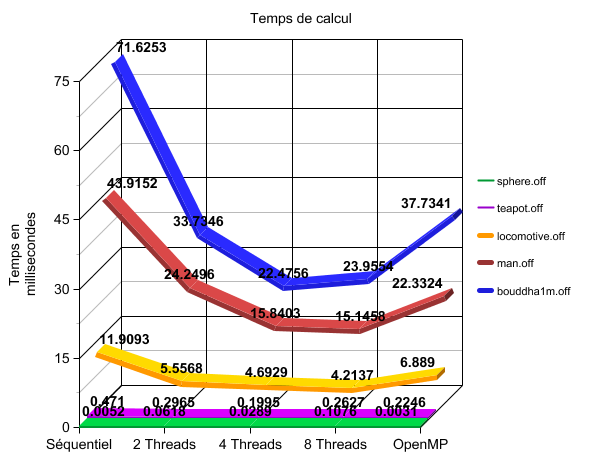
\includegraphics[scale = 0.7]{graph_execTime_machine1.png}
	\end{center}
\section{Conclusion}
% Conclusion et conjecture

\newpage
\bibliographystyle{unsrt}
\bibliography{biblio}

\end{document}
